\documentclass{article}[a4paper]

\usepackage{subfigure}
\usepackage{graphicx}
\usepackage{amsmath}
\usepackage{textcomp}

\title{Beamforming}

\begin{document}

\maketitle

\section*{Introduction}

An underwater habitat connects wirelessly to a ship on the surface by means of ultrasonic hydrophones installed at the top of the habitat. In order to increase communications range, multiple hydrophones can make a beamforming system. A flat rectangular area, 45 cm x 45 cm in dimension, is provisioned. The area lies in the y-z plane of reference coordinate system, as depicted in Figure \ref{fig:coord}.
\begin{figure}[h!]
   \centering
   
\includegraphics[width=0.4\textwidth]{coord.png}
   \caption{Reference coordinate system with available beamformer area}
   \label{fig:coord}
\end{figure}

Hydrophone operates in frequency range of 20 kHz to 90 kHz. The communication link uses a carrier frequency of 30 kHz. Hydrophone has a cosine radiation pattern, described by expression
\[ D(\phi,\theta) = \cos^2(\theta) \]
with $\phi$ being azimuth angle, and $\theta$ elevation angle. The radiation pattern is presented in the reference coordinate system in Figure \ref{fig:hydrophone}.
\begin{figure}[h!]
   \centering
   \subfigure[3D view]{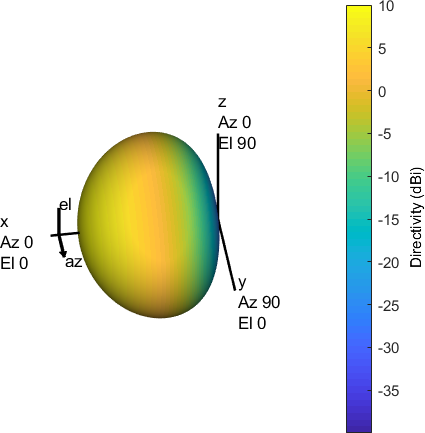
\includegraphics[width=0.415\textwidth]{hydrophone_3d.png}}
   \hfill
   \subfigure[Azimuth cut at 0deg]{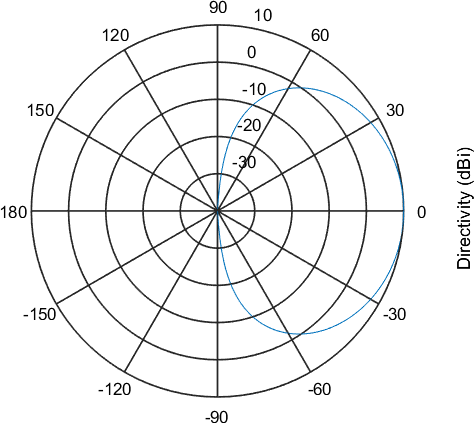
\includegraphics[width=0.45\textwidth]{hydrophone_cut.png}}
   \caption{Radiation pattern of a hydrophone element}
   \label{fig:hydrophone}
\end{figure}
Physically, hydrophones are circular, 5 cm in diameter. All hydrophones in the beamforming system are installed with their radiation maximum pointed to zenith, i.e. perpendicular to sea surface. At the other end, the ship is equipped with a single hydrophone mounted on ship's hull, and pointing at nadir, i.e. perpendicular to seabed.

Consider the signal narrowband. The ship is in the farfield of the beamforming system. Assume the communication link is being established in the Adriatic sea, with average salinity of 38\textperthousand, and sea temperature of 20\textdegree.

\pagebreak

\section*{Task 1}

Design a single linear antenna array to achieve the best link between the habitat and the ship in four given scenarios.
\begin{description}
	\item[Scenario 1] The ship is directly above the beamforming system.
	\item[Scenario 2] The ship is located along the longitudinal (y) axis of the beamforming system, at an elevation of 30\textdegree.
	\item[Scenario 3] The ship is located along the longitudinal (y) axis of the beamforming system, at an elevation of 60\textdegree.
	\item[Scenario 4] The ship is located along the longitudinal (y) axis of the beamforming system, at an elevation of 70\textdegree.
\end{description}

\begin{figure}[h!]
   \centering
   \subfigure[Scenario 1]{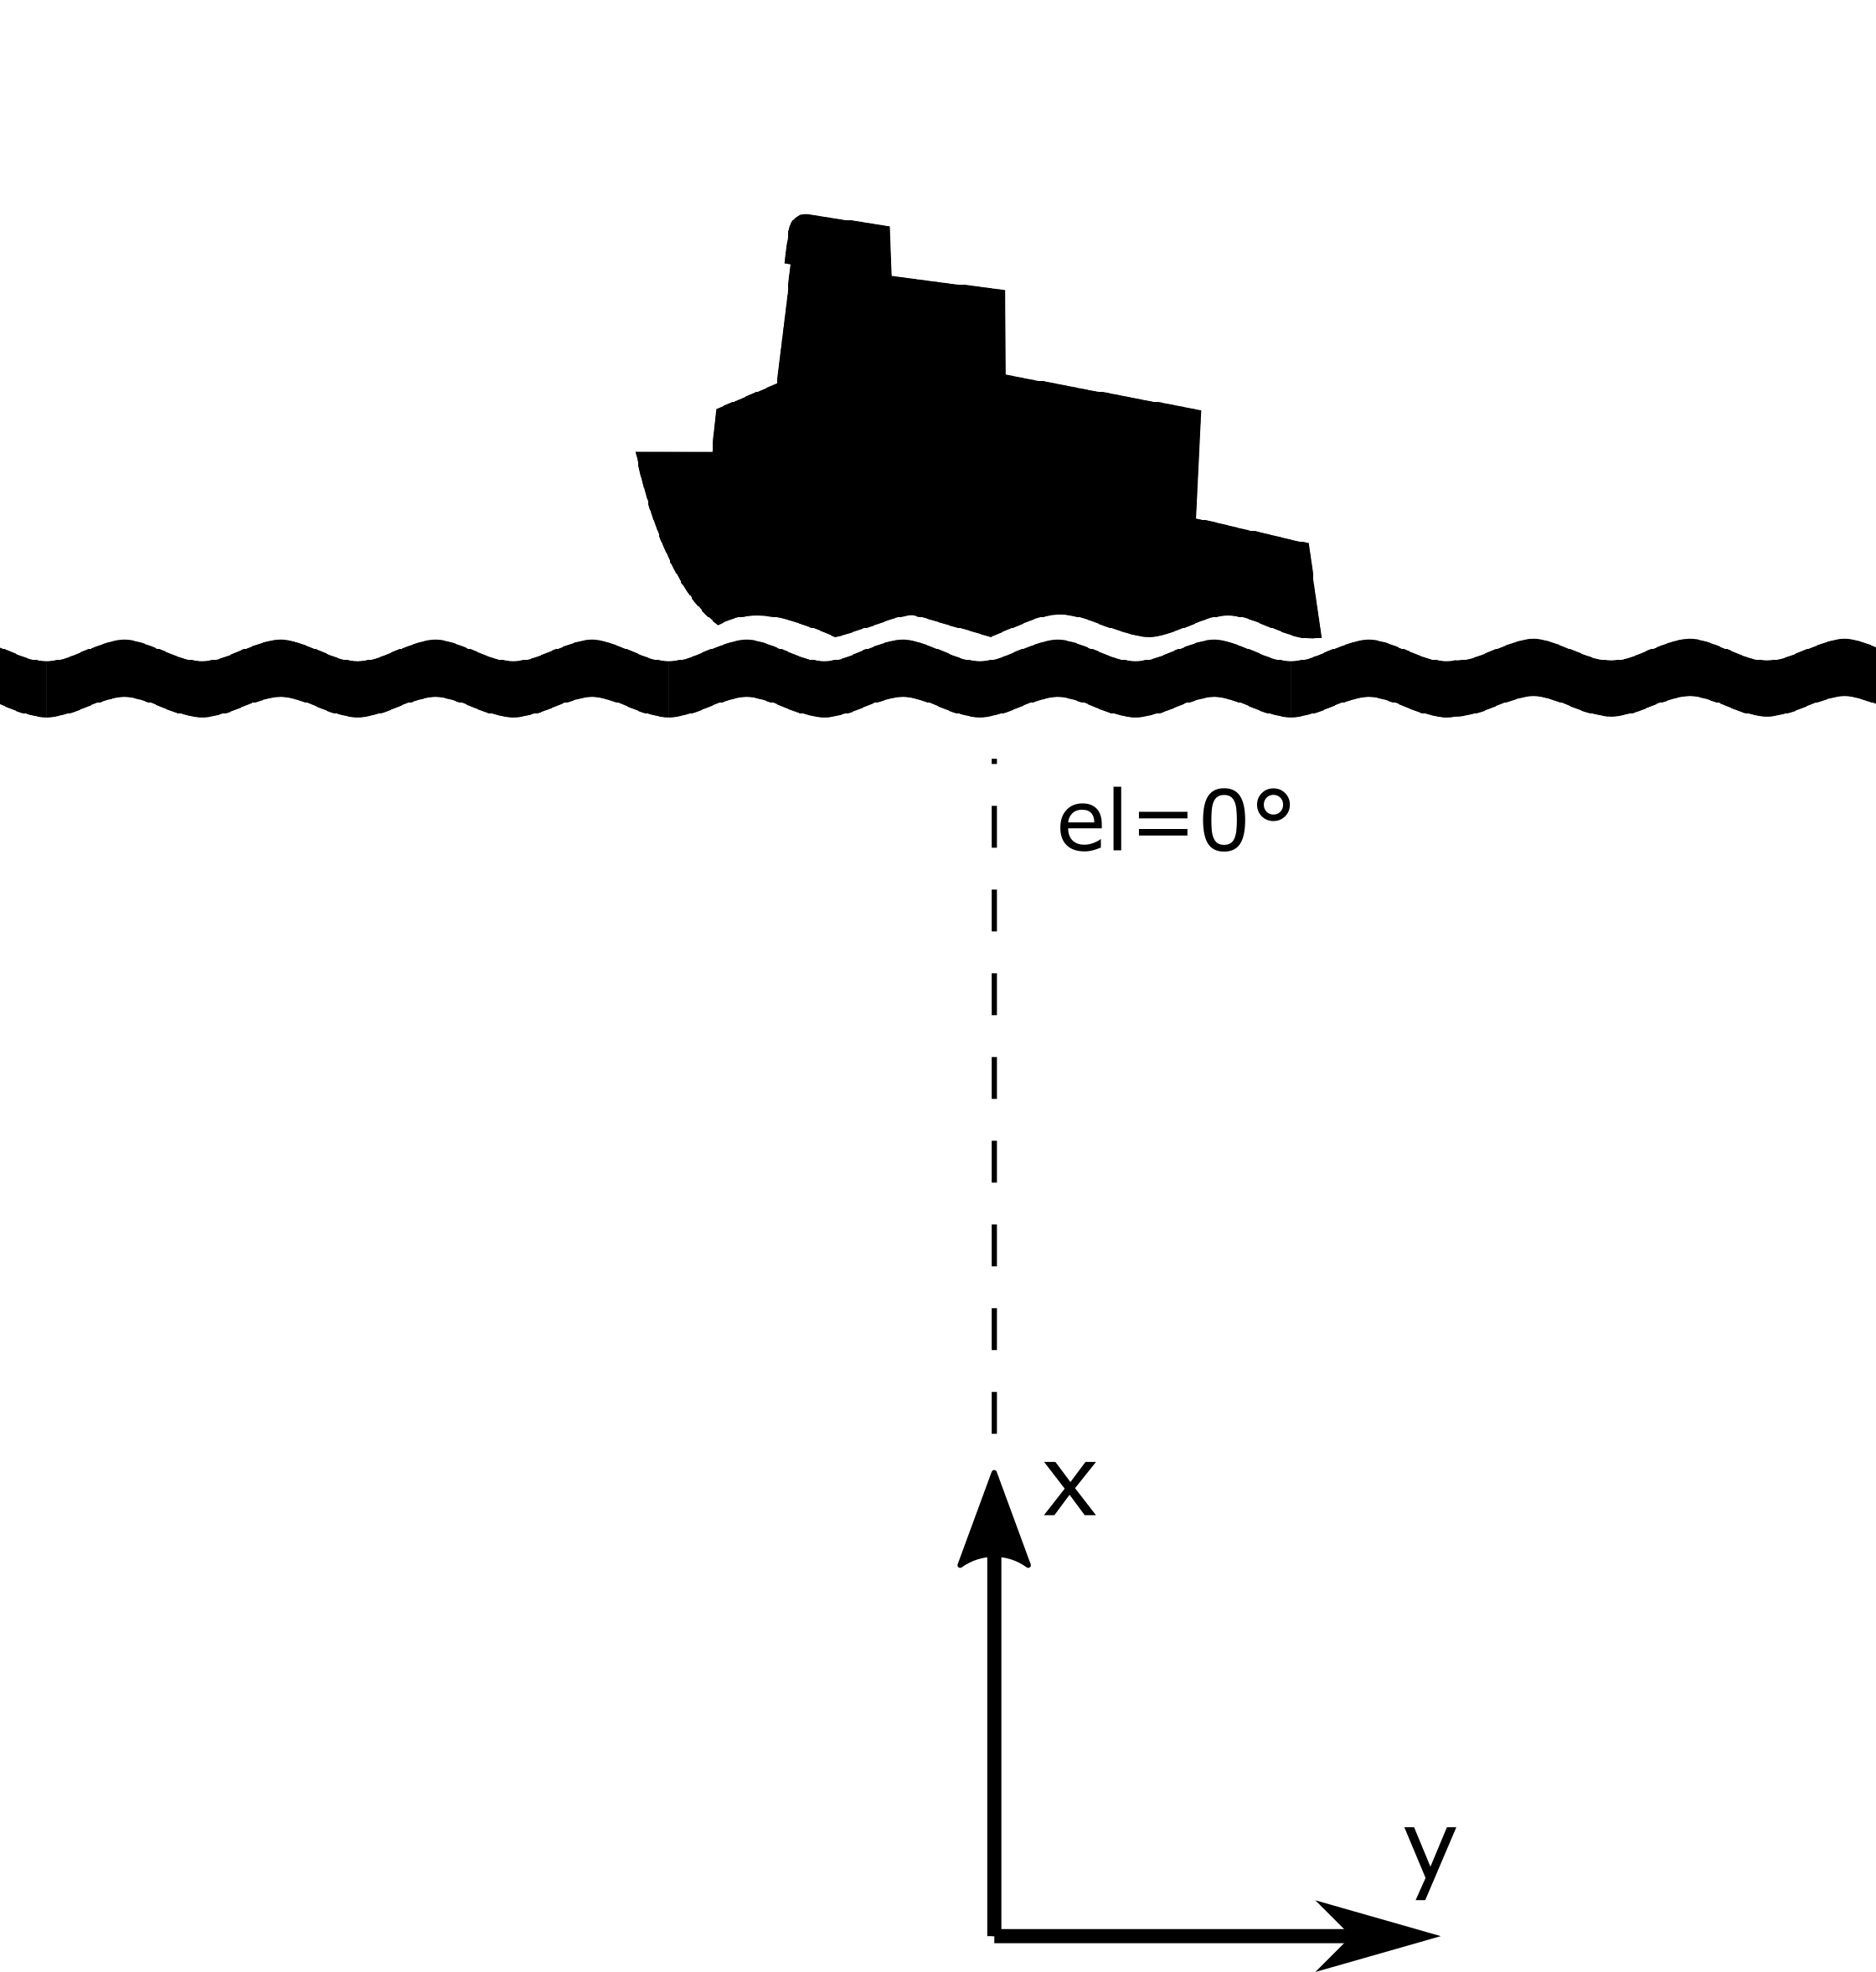
\includegraphics[width=0.45\textwidth]{scenario1.png}}
   \hfill
   \subfigure[Scenario 2]{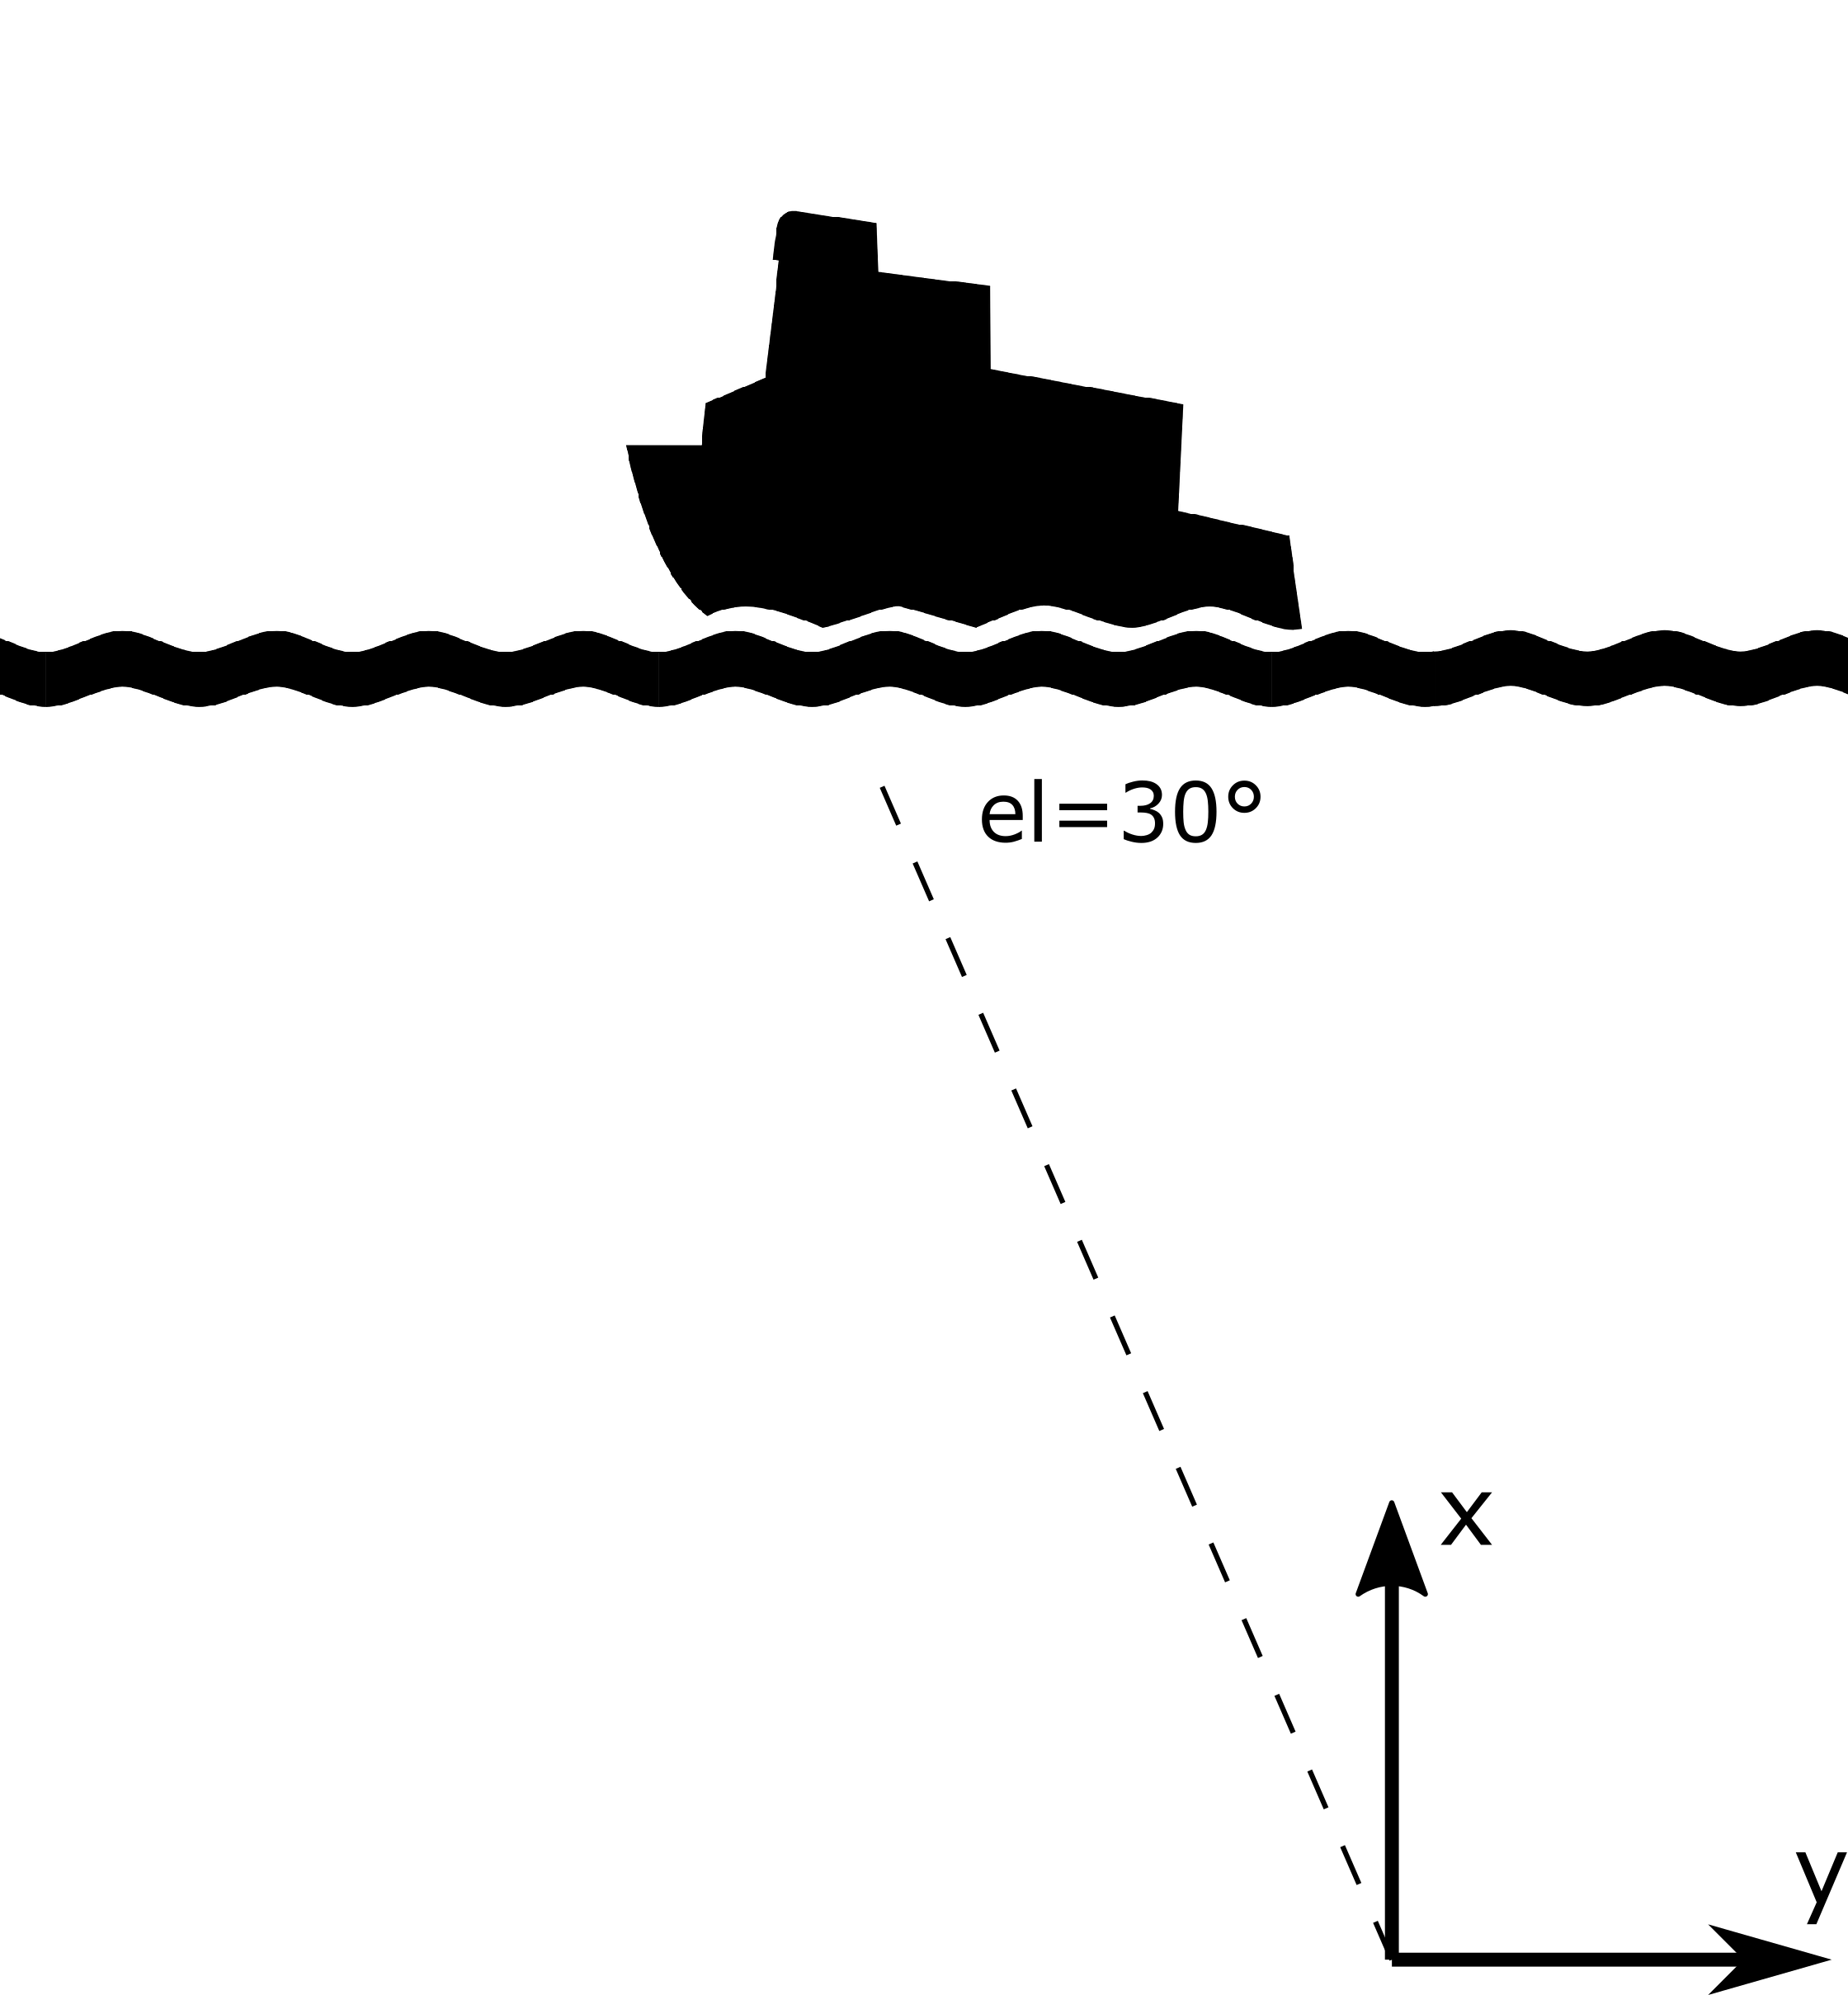
\includegraphics[width=0.45\textwidth]{scenario2.png}}
   \\
   \subfigure[Scenario 3]{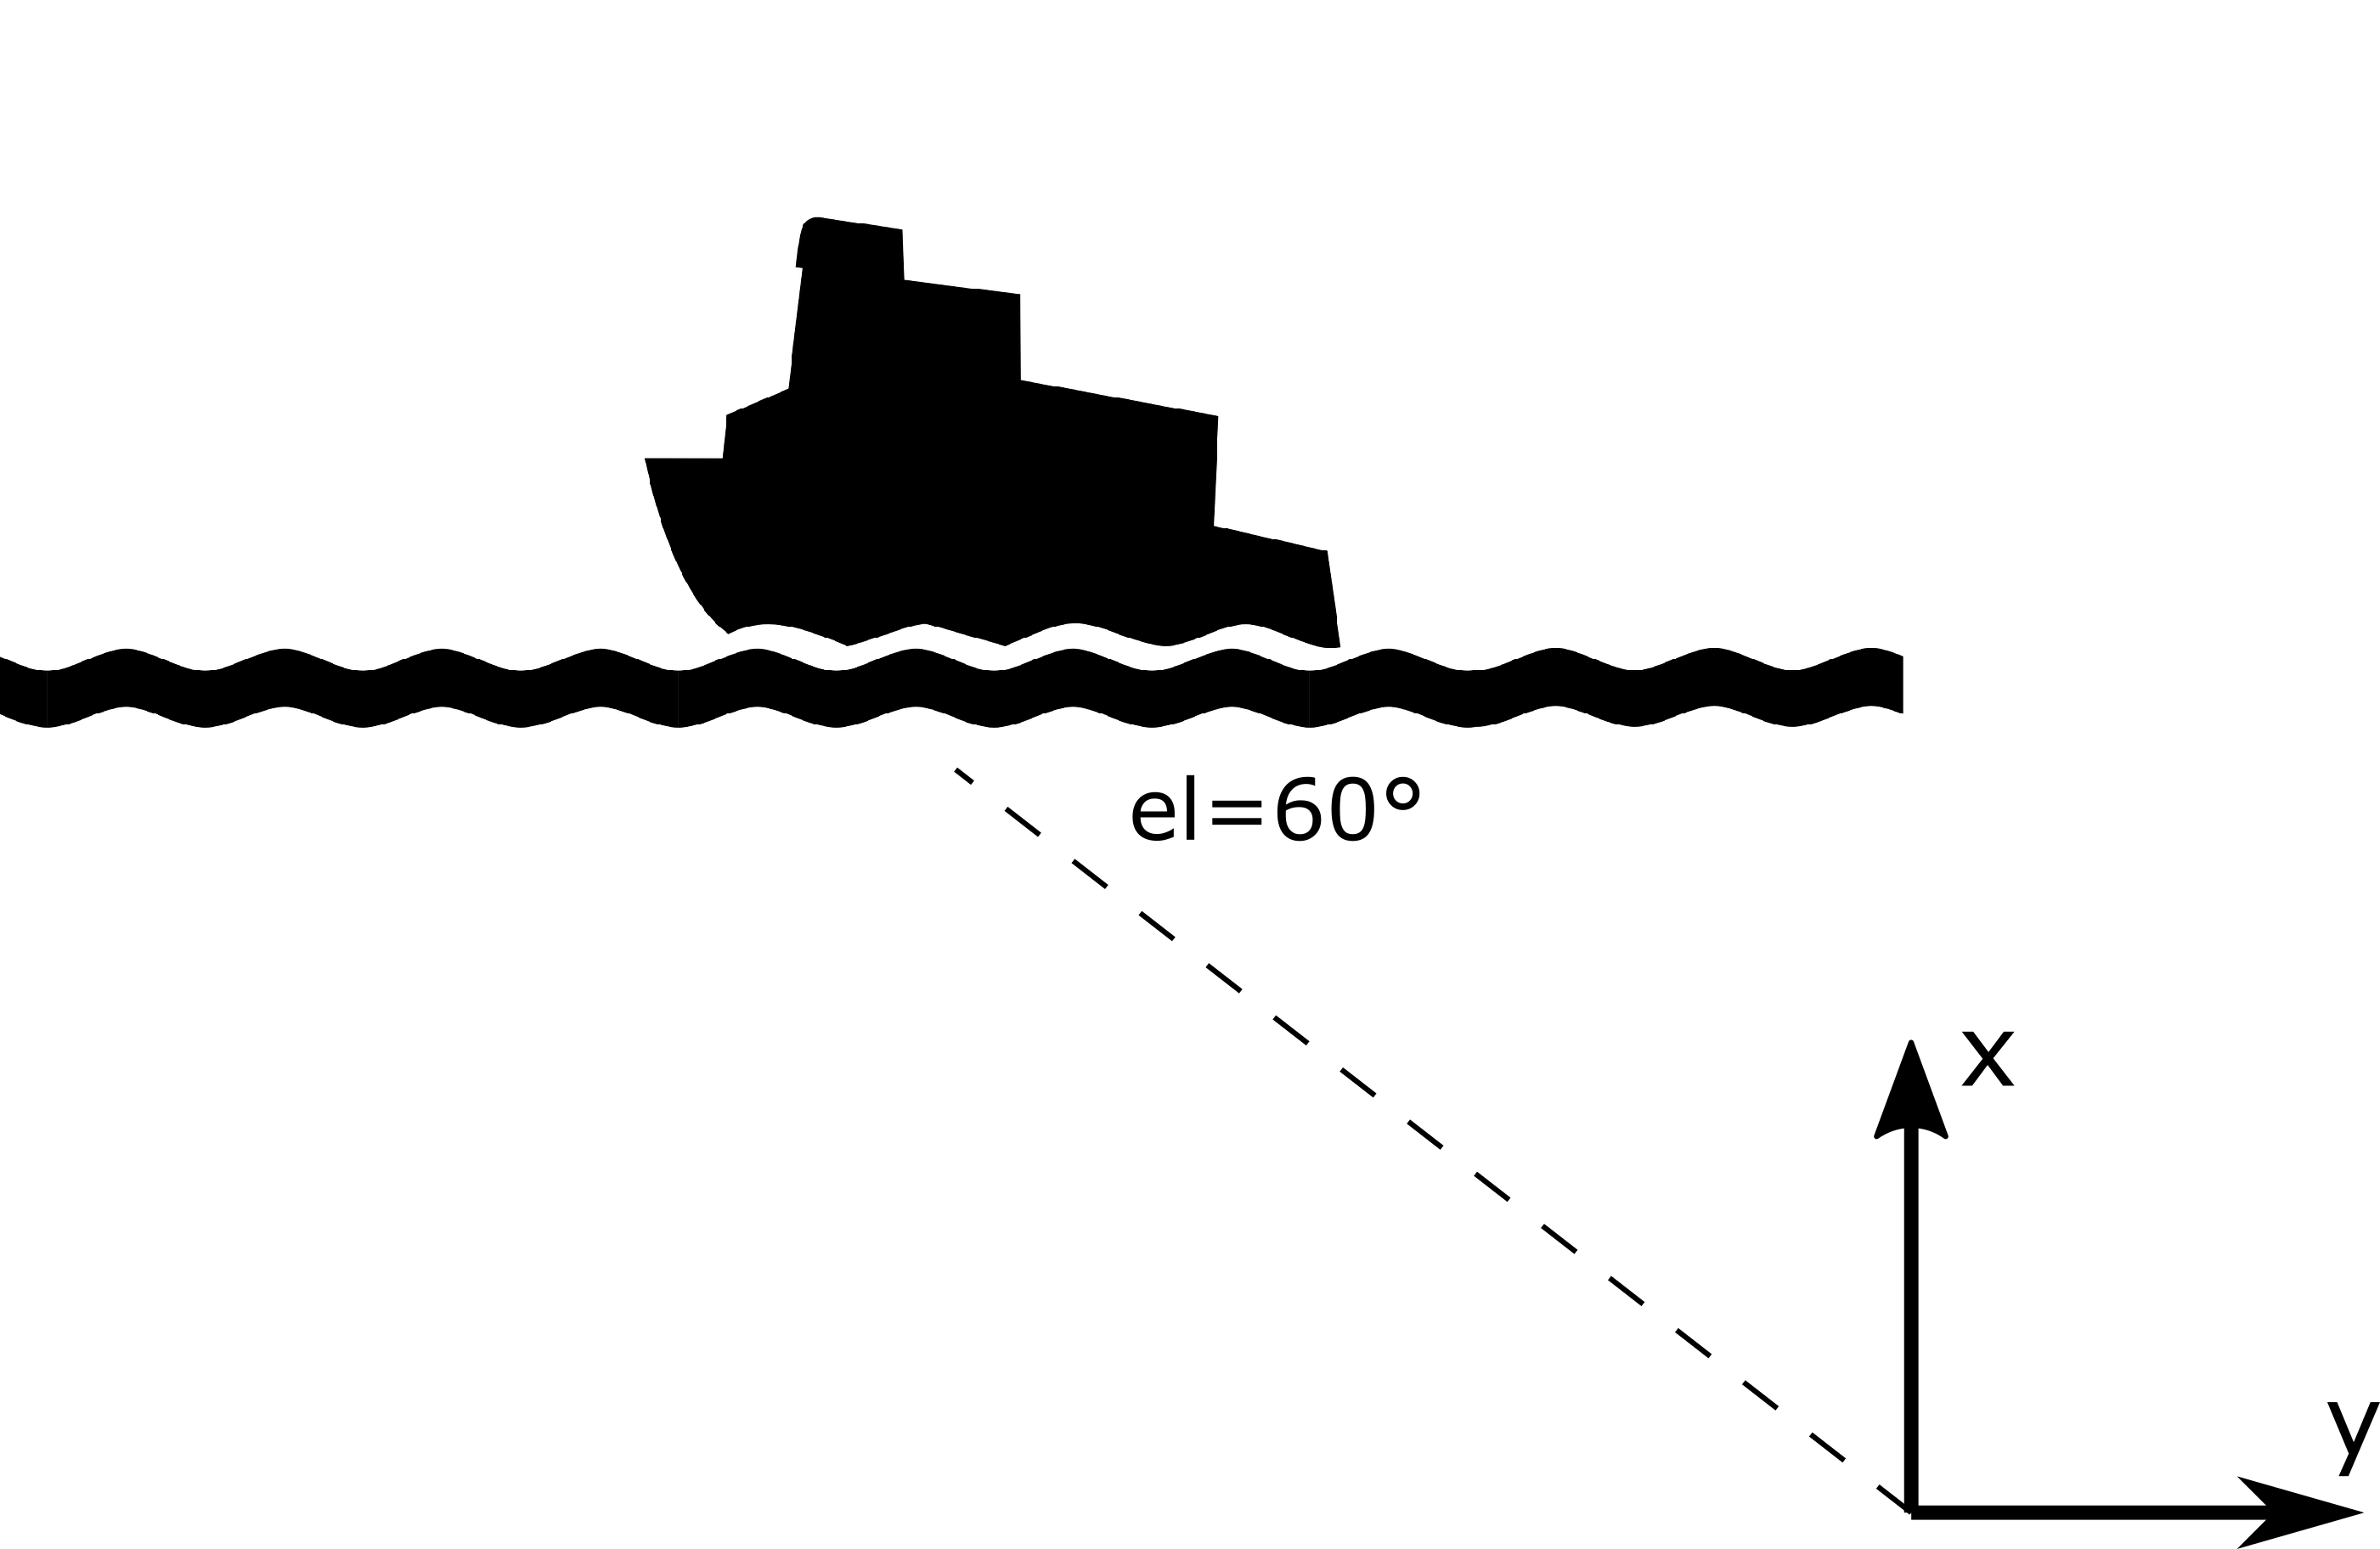
\includegraphics[width=0.45\textwidth]{scenario3.png}}
   \hfill
   \subfigure[Scenario 4]{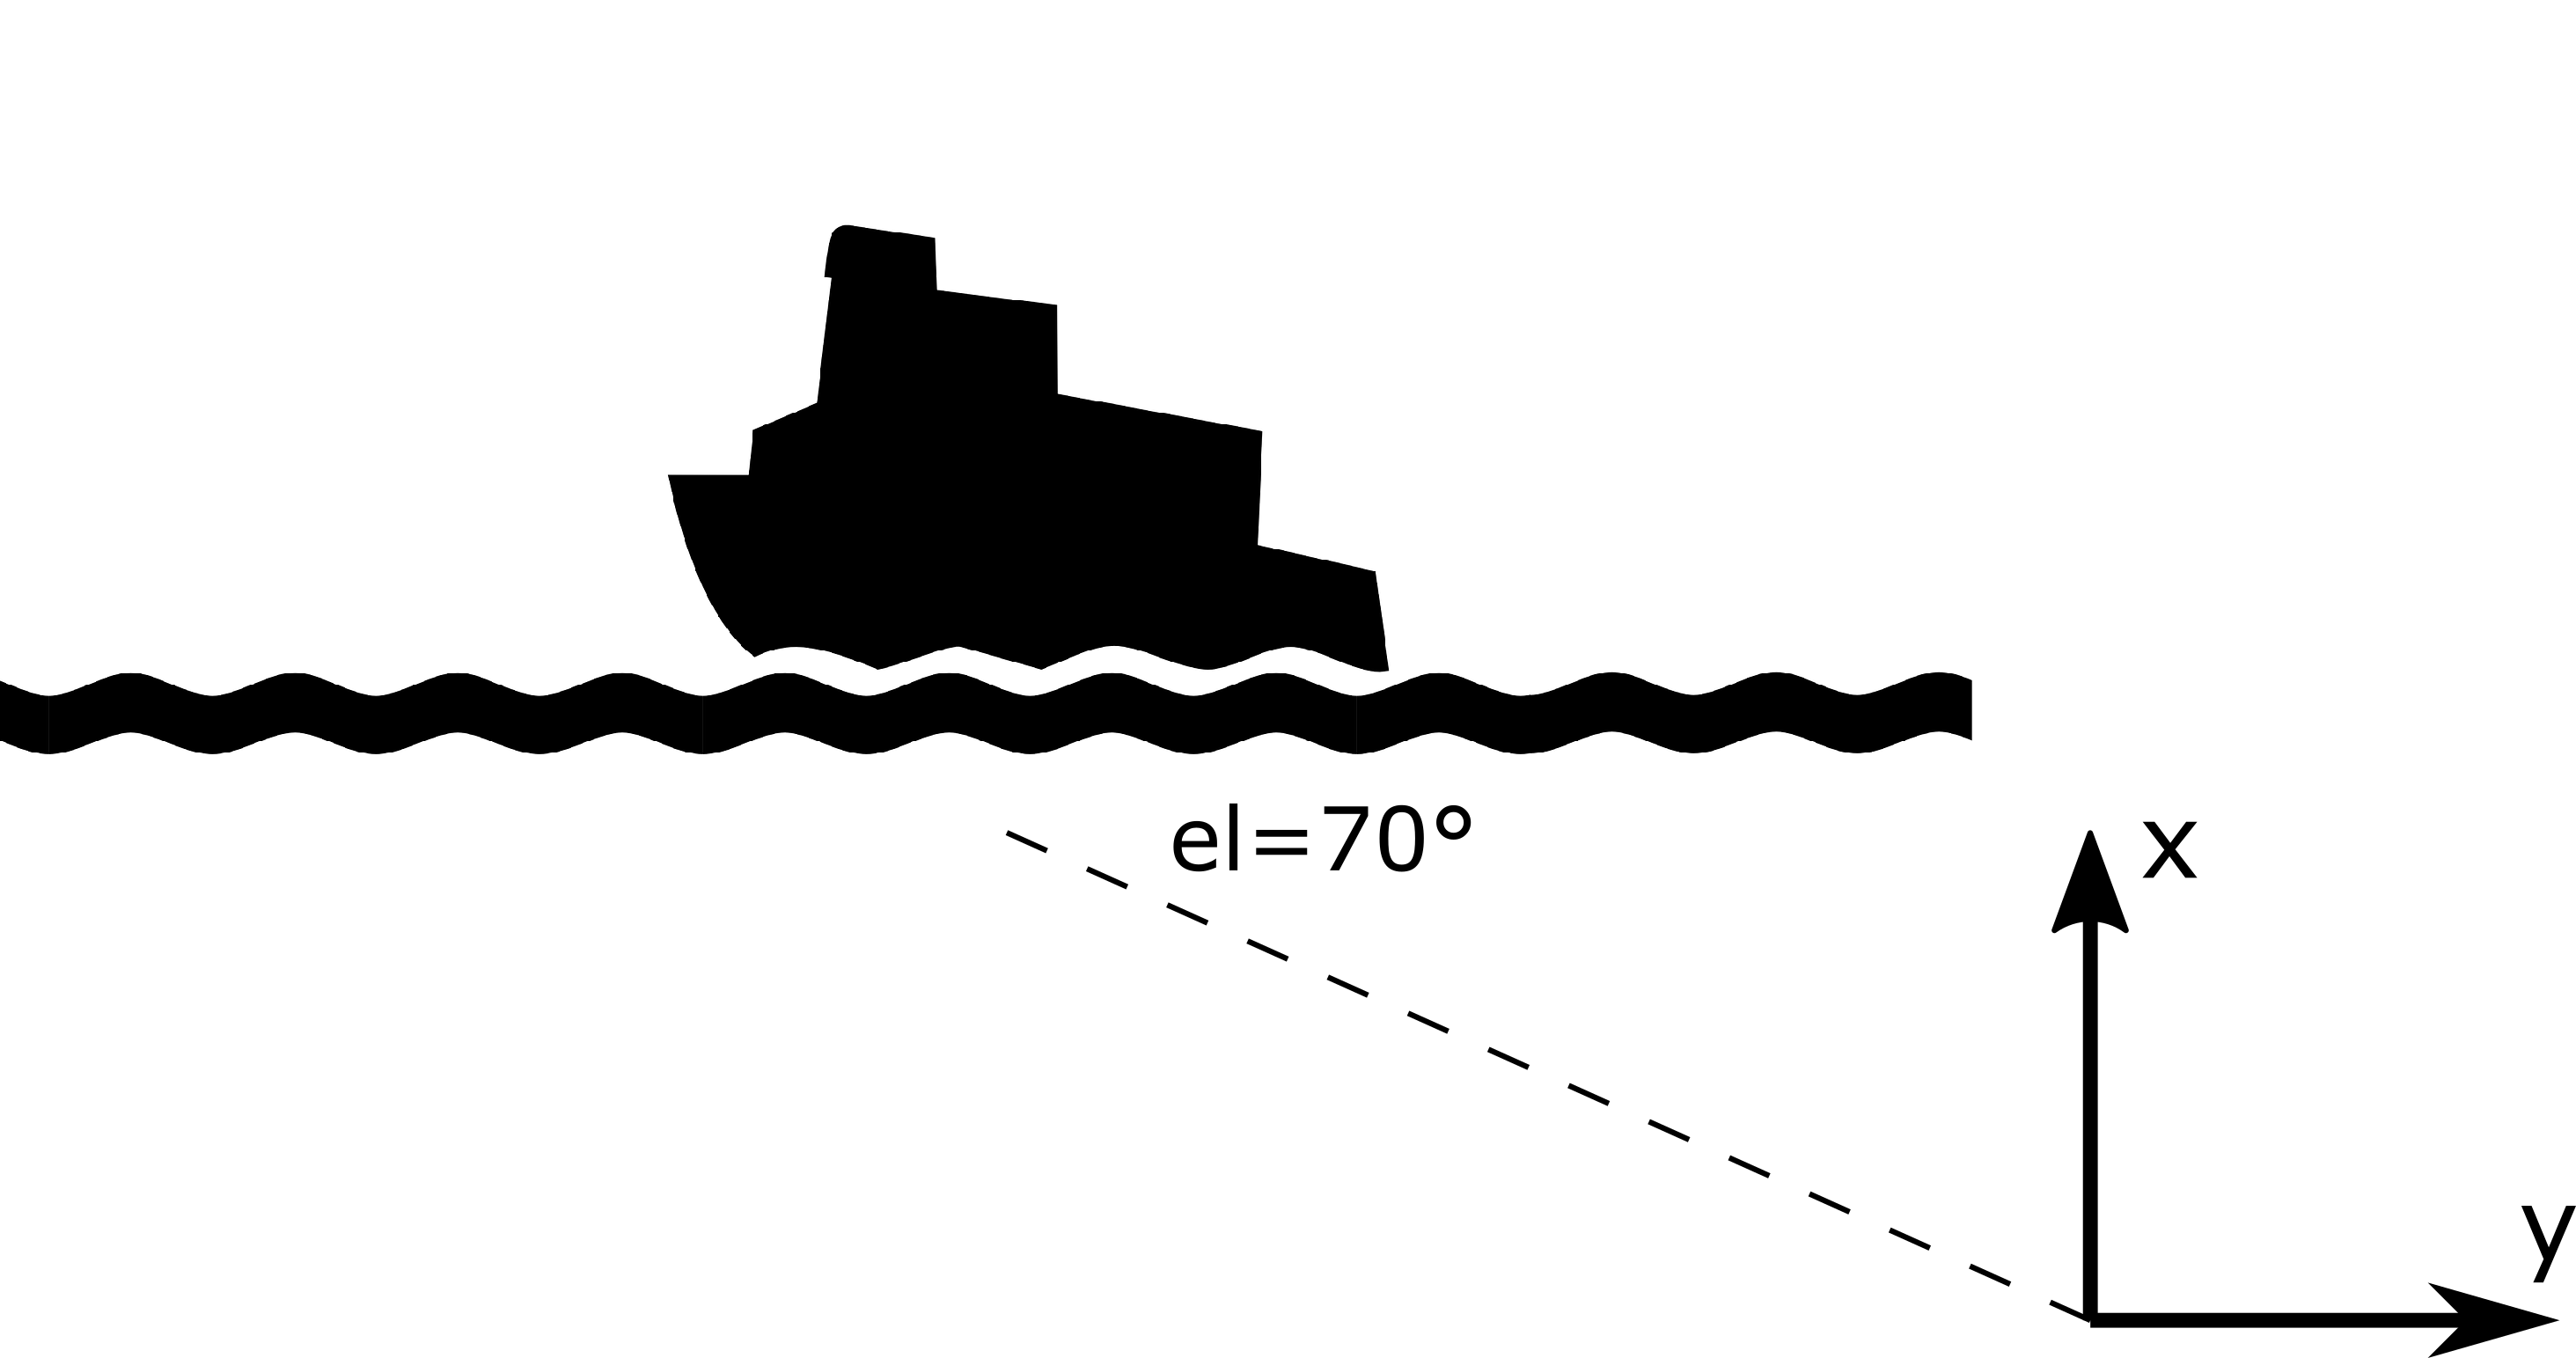
\includegraphics[width=0.45\textwidth]{scenario4.png}}
   \caption{Scenarios for Task 1}
\end{figure}

Elevation angle is considered from beamforming system's normal.

A beamforming system is defined by giving y coordinates of each hydrophone element. Number of elements is arbitrary, given the limitations introduced in Introduction. For each of the four scenarios, provide complex weights that are applied to each of the hydrophone elements to achieve optimal beamforming for the particular scenario.

\subsection*{Output data}

\begin{description}
	\item[task1\_elements.csv] \,\\ The file contains a one-dimensional array representing the position of each hydrophone element along the y axis in metres.
	\item[task1\_scenarioX.csv] \,\\ The file contains a one-dimensional array of complex numbers representing the weights applied to each hydrophone element. Weights are given for elements in the same order as defined in task1\_elements.csv. Array length is equal to the number of elements in the beamforming system. All numbers are inside, or at the edge of the unit circle.
\end{description}

\subsection*{Scoring}

The beamforming system you designed is evaluated for each of the given scenarios. For the first three scenarios, points are awarded for the directivity the beamforming system achieves in the direction of the ship, after applying the given beamforming weights. If the ship is in the main lobe of the beamforming system, the number of awarded points is equal to
\[ D_\textrm{target} - \varDelta \phi \]
where $D_\textrm{target}$ is the directivity in the direction of the ship, and $\varDelta \phi$ the angular distance between the ship and the direction of beamformer's maximum directivity in degrees. If the ship is within the strongest sidelobe of the beamforming system, the number of awarded points is equal to
\[ D_\textrm{target} - \dfrac{\varDelta \phi}{10} \]
The ship is considered to be within a radiation lobe if it is within 6 dB drop-off of the considered radiation lobe.

In scenario 4, the beamforming system is evaluated with the given beamforming weights, and its directivity compared to that of the same beamforming system with uniform excitation. The points are then awarded as
\[ D_\textrm{target,weighted} - D_\textrm{target,uniform} \]
The highest number of points for this scenario is 15.

For all scenarios, the following rules apply: A beamforming system constructed with just one element is awarded no points. A beamforming system acheiving negative directivity in the direction of the ship is awarded no points. Directivity is consided in units dBi. Negative points are not awarded (nor penalized :) ).

After evaluating the task for both teams, the total number of points is normalized to the best team. Hence, the best team is pondered to 50 points, and the points for other teams is linearly scaled accordingly.

\end{document}